
\chapter{安装}
\label{chap:installation}

\begin{flushleft}
\rule[0mm]{\textwidth}{.1pt}
\end{flushleft}

使用Slackware前,当然要先获取Slackware并进行安装。不论是购买Slackware
的CD或是从网上免费下载都是很容易的。只要对自己的电脑有一定的基础知识,
并且想进一步学习,安装Slackware是非常容易的。安装程序本身就像是一步一
步进行的。因此,我们很快就能熟悉这个过程并快速地运行它。事实上,
Slackware鼓吹自己是所有功能完善的Linux发行版中安装时间最短的版本之一。

\section{获取Slackware}
\label{sec:installation:gettingSlackware}

\subsection{官方CD及套装}
\label{sec:installation:gettingSlackware:official}

官方的Slackware CD套装可以从Slackware公司得到。CD套装包含6个
CD\footnote{这里以Slackware 13.37为例,参见
\url{http://slackware.com/getslack/torrents.php}},第一张CD包含基本安装
所需要的所有软件,具体包括A/AP/D/E/L/N系列及可启动的安装器,内核,
testing/,及Slackwbook。第二张CD包含一些文档及X系统,具体包括
F/K/T/TCL/X/XAP/Y、L系列的源码及/testing kernel source。第三张CD含有
KDE系列及A/AP/E/F/安装器的源码。第四张CD含有KDEI、/extra软件包及D系列的
源码。第五张CD含有KDE/XAP系列的源码。第六张CD包含/pasture软件包、
K/N/T/TCL/X/Y的源码及USB和PXE的安装器。

你也可以购买一个套装,其中含有6个CD及Slackbook的印刷版,还有一些简洁的
Slackware工具,可供你显摆你作为geek的自尊。我们倾向于通过Slackware
store来从网上购买Slackware商品。

\url{http://store.slackware.com}

你也可以通过打电话或发邮件来订购。

\begin{table}[htpb]
  \centering
  \begin{tabular}{c|l}
    \hline\hline 
  方式 & 详细联系信息  \\ \hline
  电话 & 1-(925)674-0783 \\
  网页 & \url{http://store.slackware.com} \\
  Email & orders@slackware.com \\
  写信 & 114 Claremont Drive, Brentwood, CA 94513 \\
  \hline \hline
  \end{tabular}
  \caption{Slackware Linux公司的联系信息}
  \label{tab:slackwareLinuxIncContactInformation}
\end{table}

\subsection{通过互联网}
\label{sec:installation:gettingSlackware:internet}

Slackware可以从网上免费下载,你也可以发送email邮件问一些支持问题,但我
们会优先考虑那些购买官方CD的人。为什么这么说呢?因为我们收到了一大堆的
邮件,但我们的时间是有限的,所以在发送email之前,请先阅读第二章的帮助。

Slakcware官网为:

\url{http://www.slackware.com}

Slackware的FTP主站为: 

\url{ftp://ftp.slackware.com/pub/slackware}

请记住,虽然我们的FTP站点是为公众开放的,但带宽有限。在下载时请优先考
虑离你近一点的镜像站下载。你可以在我们的网址上找到一个镜像站列表:

\url{http://www.slackware.com/getslack}

\section{系统要求}
\label{sec:installation:systemRequirements}

一个简单安装的Slackware的最小要求\footnote{这是Slackbook 2的内容,对于
  Slackware 13.37不知是否还适用。}如下:

\begin{table}[htpb]
  \centering
  \begin{tabular}{c|c}
    \hline \hline 
    硬件各类 & 具体要求 \\ \hline
    处理器 & 586架构以上 \\
    内存 & 32MB以上 \\
    硬盘空间 & 1GB以上 \\
    多媒体驱动器 & 4倍速的CD-ROM以上 \\
    \hline\hline
  \end{tabular}
  \caption{系统要求}
  \label{tab:systemRequirements}
\end{table}
如果你有可启动的CD盘,那么就不需要软盘驱动器了。当然,这表明如果你没有
光盘驱动器,那么你就得有一个软盘驱动器来进行网络安装。如果采用NFS方式
安装的话,还需要一张网卡。请参见NFS一节获取更多信息。另外,如果你并不
是在全新的系统上安装Slackware,还可以采用从硬盘安装。

声称只要1G的硬盘有点狡猾了。因为对于最小安装而言1G空间是可以的,但如果
你是采用完全安装,那么至少要有2GB的硬盘空间\footnote{Slackware 13.37的
  完全安装需要5.6GB左右},另外还得准备出存放私人文件的硬盘空间。多数用
户并不采用完全安装,事实上,许多人在只有100MB硬盘空间的机器上运行
Slackware。

Slackware可以安装到内存少,硬盘小或CPU落后的系统上,但如果这么做,就要
付出点代价。如果你正面临这样的情况,那么可以查看CD上的
\texttt{LOWMEM.TXT}文件,它包含了一些有用的信息。

\subsection{软件包系列}
\label{sec:installation:systemRequirements:series}

由于要求简洁的原因,历史上Slackware被分为软件系列。那时候,人们要想连
接到FTP服务器上,只能通过奇慢无比的波特率300的调制解调器,所以
Slackware被拆分成不同的集合,而这些集合的大小适合存放于软盘上,所以用
户只需要下载和安装他们感兴趣的软件集合。今天,Slackware中使用软件包系
列的目的,主要是用来对软件包进行分类。用软盘安装的日子已不复存在。下面
是对软件包系列的一个简要描述。

\begin{table}[htpb]
  \centering
  \begin{tabular}{l|l}
    \hline \hline
    系列 & 内容 \\ \hline
    A & \parbox[t]{0.8\textwidth}{基本系统,其中包含的软件足以让我们启
动并运行一个系统,且有一个文本编辑器及基本的通信软件} \\
    AP & 一些不需要X Window系统的应用软件。\\
    D & 软件开发工具。包括编译器、调试器、解释器及man手册等。\\
    E & GNU Emacs\\
    F & FAQ、HOWTO及其它一些文档。\\
    K & 内核源码。\\
    KDE & \parbox[t]{0.8\textwidth}{KDE桌面环境。一个外观类似MacOS及
Windows的X桌面环境。其中还包含作为KDE依赖的Qt库。}\\
    KDEI & KDE桌面的国际化语言包\\
    L & 库文件。其它程序要用到的动态链接库。\\
    T & teTex文档系统。\\
    TCL & 工具命令语言。包括Tk、TclX及TkDesk等。\\
    X & 基本的X Window系统\\
    XAP & 主要桌面环境中不包含的一些X应用程序(如Ghostscript及firefox
    等)。\\
    Y & BSD控制台游戏。\\
    \hline\hline
  \end{tabular}
  \caption{软件包系列}
  \label{tab:softwareSeries}
\end{table}

\subsection{安装方法}
\label{sec:installation:systemRequirements:methods}
本节中介绍有一些方法相当古老,笔者只尝试过CD/DVD安装及硬盘安装,其它都
没试过,只能照书翻译。
\subsubsection{软盘}
\label{sec:installation:systemRequirements:methods:floppy}
早先的时候是可以通过软盘的方法安装Slackware的,但随着软件包的增大(是的,
一些单独的软件在增大),软盘的方法已经不得不被淘汰了。最后一个能用软盘
安装的版本是Slackware 7.1的部分安装。A系列和N系列几乎可以完全安装,这
就提供了安装该发行版其它软件的一个基础系统。如果你考虑使用软盘安装(尤
其在老的硬件上),那么我们推荐用其它的方法安装或者用Slackware老的版本。
Slackware 4.0和7.0在这种情况下还是很可靠的。

注意,如果你想采用CD安装,但却没有可启动的CD,那么还是需要软盘的,同样,
对NFS安装也如此。

现在多数的电脑连软驱都没有了,更别说软盘了,如果你是一个新手,完全不用
考虑这种方法,当然,老手也几乎不需要考虑。

\subsubsection{光驱}
\label{sec:installation:systemRequirements:methods:cdrom}

可启动的CD可以在Slackware Linux公司的官网上获得(参见获取Slackware这一
节)。采用基于CD/DVD的安装全更容易一些。如果你没有可启动CD的话,那就需
要从软驱启动了。另外,如果你的硬件使用启动CD上的内核有问题的话,你也可
能需要使用特制的软盘了。

对于Slackware 8.1版本,我们使用了一种新的方法制作启动CD,这种方法对于
一些特定的BIOS芯片工作得不太好(相比于当前多数Linux CD遇到的问题而言,
这个问题简直不值一提)。如果你遇到这种情况,我们还是建议你使用软盘启动。

第\ref{sec:installation:systemRequirements:methods:bootDisk}节和第\ref{sec:installation:systemRequirements:methods:supplementalDisk}节提供了关于选择及创建启动软盘的信息,也许会很有用。

\subsubsection{NFS}
\label{sec:installation:systemRequirements:methods:nfs}

NFS(the Network File System 网络文件系统)是一个远程机器上使用的文件
系统。NFS安装使我们可以从网络上的另一台机器上安装Slackware。作为获取源
的那台机器要为安装机导出Slackware发行版的目录树。当然,这需要关于NFS的
一定知识,在第\ref{sec:networkConfiguration:networkFileSystem}节中有介
绍。NFS可以通过PLIP(parallel port并行端口)、SLIP及PPP(一个调制解调
器连接)进行安装。然而,我们建议最好通过网卡进行连接。毕竟通过打印机端
口来安装一个操作系统是非常非常慢的。

\subsubsection{启动盘}
\label{sec:installation:systemRequirements:methods:bootDisk}

软盘已经几乎被淘汰,这里按slackbook 2进行翻译,以防某些万一需要的情况。
Slackware 13.37的光盘已经明确写明,不再支持使用其中的内核制作启动盘了。

所谓启动盘指的是一张软盘,通过它我们真正启动并开始安装。它包括一个压缩
的内核镜像,用来在安装过程中控制硬件。因此,这是必须要有的(除非你是从
CD启动,就像在光驱这一节中讨论的一样)。启动盘镜像位于
\texttt{bootdisks/}目录下。

Slackware中,可以选择不止一个启动盘(具体而言是16个。)。在文件
\path{bootdisks/README.TXT}中有所有启动盘的完整列表及对应的描述。然
而,多数用户可以使用\texttt{bare.i}(IDE设备使用)或
\texttt{scsi.s}(SCSI设备用)的启动盘镜像。

参见第
\ref{sec:installation:systemRequirements:methods:makingTheDisks}节以获
取关于从镜像制作启动盘的介绍。

启动之后,会有提示要求插入根磁盘。我们建议你按照启动盘的提示进行。
\subsubsection{根磁盘}
\label{sec:installation:systemRequirements:methods:rootDisk}

这节的内容也是被淘汰的。

根磁盘包含了setup程序及安装过程中使用的一个文件系统。这个也是必须的。
根磁盘镜像位于\texttt{rootdisks/}文件夹下。我们需要从
\texttt{install.1}及\texttt{install.2}两文件制作两个根硬盘。在这个目录
下,你还可以找到\texttt{network.dsk}、\texttt{pcmcia.dsk}、
\texttt{rescue.dsk}及\texttt{sbootmgr.dis}的磁盘镜像。

\subsubsection{追加盘}
\label{sec:installation:systemRequirements:methods:supplementalDisk}

如果你执行的是NFS安装或安装系统中带有PCMCIA设备,那么你需要一个追加盘。
追加盘的镜像也是在\texttt{rootdsks/}文件夹下,文件名为
\texttt{network.dsk}及\texttt{pcmcia.dsk}。近来也追加了
\texttt{rescue.dsk}及\texttt{sbootmgr.dsk}盘。急救盘是一个安装在软盘上
的,可以在4MB内存上运行的一个根磁盘镜像。它包含了一些基本的网络工具及
vi编辑器,我们可以用它在一个破坏了的系统上进行快速的修复。
\texttt{sbootmgr.dsk}是用来启动其它设备的。

根磁盘在加载之后会指示你使用其它的追加盘的。

\subsubsection{制作启动盘}
\label{sec:installation:systemRequirements:methods:makingTheDisks}
选择好了启动盘镜像,就需要将它放到软盘中,根据使用的操作系统的不同,这
个过程也有一些小差别。如果运行的是Linux(或其它类Unix的操作系统),你
需要使用\texttt{dd}命令,假设使用的是\texttt{bare.i}镜像文件,软驱对应
的设备文件是\texttt{/dev/fd0},那么制作\textbf{bare.i}软盘的命令为

\begin{Verbatim}[frame=single, commandchars=\\\{\}]
\% \textbf{dd if=bare.i of=/dev/fd0}
\end{Verbatim}

如果运行的是Microsoft的操作系统,你需要使用\texttt{RAWRITE.EXE}程序,
在我们的发行版中也包含了该程序,它与软盘镜像在同一个文件夹下。同样的,
假设用的是\texttt{bare.i}镜像,软驱为\texttt{A:},在DOS提示符下,输入
下面的命令即可。
\begin{Verbatim}[frame=single, commandchars=\\\{\}]
C:\textbackslash{} \textbf{rawrite a: bare.i}
\end{Verbatim}
\section{启动安装器}
\label{sec:installation:bootingTheInstaller}
启动安装器很简单,只要将Slackware安装盘插入你的CD或DVD驱动器,之后重启
就行了。另外,你可能要先进入BIOS修改启动顺序,把光驱的启动顺序放在硬盘
的启动顺序之前。有一些计算机可以在系统启动时,按下某些键来动态的改变启
动顺序。由于每台电脑都是不同的,我们不可能为所有的电脑提供一个修改启动
顺序的说明,但修改的方法在几乎所有的机器上都是很容易的。

一旦你的电脑从CD启动了,你就会被带到一个界面,要求你输入特定的一些内核
参数,从这里开始,你就可以像使用急救盘那样使用这个安装器了。一些系统可
能要求特定的内核参数才能启动。但这是极少数的情况,多数情况下,只要按下回
车键,启动内核就可以了。

\begin{Verbatim}[frame=single]
Welcome to Slackware version 13.37 (Linux kernel 2.6.37.6)!

If you need to pass extra parameters to the kernel, enter them at the prompt
below after the name of the kernel to boot (huge.s etc).

In a pinch, you can boot your system from here with a command like:

boot: huge.s root=/dev/sda1 rdinit= ro 

In the example above, /dev/sda1 is the / Linux partition.

This prompt is just for entering extra parameters.  If you don't need to enter
any parameters, hit ENTER to boot the default kernel "huge.s" or press [F2] 
for a listing of more kernel choices.
\end{Verbatim}
启动过程中,你应该会看到屏幕上刷了一排排了文字。不必惊慌,这是很平常的。
这是内核启动过程中,对硬件进行检测并准备载入操作系统(现在载入的是安装
器)时产生的信息。如果你感兴趣的话,之后可以用\texttt{dmesg(1)}来阅读
这些信息。通常,如果你的硬件有问题,这些信息对于排除问题是十分重要的。
一旦内核完成对硬件的检测,屏幕上的信息就会停下,让你选择对非标准美式键
盘的支持。
\begin{Verbatim}[frame=single]
<OPTION TO LOAD SUPPORT FOR NON-US KEYBOARD>

If you are not using a US keyboard, you may not load a different
keyboard map.  To select a different keyboard map, please enter 1
now.  To continue using the US map, just hit enter.

Enter 1 to select a keyboard map: _
\end{Verbatim}
输入\textbf{1}并输入\textbf{Enter(回车)},就能看到一张键盘映射表。选
择符合你的键盘类型的那一项就可以继续了。
\begin{Verbatim}[frame=single,commandchars=+\[\]]
Welcome to the Slackware Linux installation disk! (version 13.37)

######  IMPORTANT!  READ THE INFORMATION BELOW CAREFULLY.  ######

- You will need one or more partitions of type 'Linux' prepared.  It is also
  recommended that you create a swap partition (type 'Linux swap') prior
  to installation.  For more information, run 'setup' and read the help file.

- If you're having problems that you think might be related to low memory, you
  can try activating a swap partition before you run setup.  After making a
  swap partition (type 82) with cfdisk or fdisk, activate it like this:
    mkswap /dev/<partition> ; swapon /dev/<partition>

- Once you have prepared the disk partitions for Linux, type 'setup' to begin
  the installation process.

- If you do not have a color monitor, type:  TERM=vt100
  before you start 'setup'.

You may now login as 'root'.

slackware login: +textbf[root]
\end{Verbatim}

其它的一些发行版会直接启动进入一个专门制作的安装程序,与之不同,
Slackware 的安装器会让你进入一个载入系统内存的轻量Linux发行版。之后,
我们就可以使用这个轻量的Linux手工运行安装程序,当然,我们也能将它作为一
个应急启动系统,在系统不能启动时对系统进行修复。现在,你已经用root登陆
了(安装器中不需要密码),这时就应该设置硬盘了。在这个节点上,如果你希
望得到一个加密的根分区,你可以安装支持RAID或LVM的软件,但这个主题已经
超出了本书的范畴。如果你希望使用这些先进的工具,我强烈建议你查看CD上的
\path{README\_RAID.TXT},\path{README\_LVM.TXT}及
\path{README\_CRYPT.TXT}文件。大多数用户并没有这种需求,因此应该直接
跳到下一步——分区。

\section{分区}
\label{sec:installation:partition}

与其它发行版不同的是,Slackware的安装器中没有使用图形化的磁盘分区工具;
而取而代之的是\texttt{fdisk(8)}及\texttt{cfdisk(8)},二者都是命令行工
具。cfdisk基于curses库\footnote{为程序提供字符终端用户接口。通俗
  地说:为字符终端(命令行)提供更好的显示,可理解为终端下的GTK等。译
  者注。},fdisk则不然。不管你用哪一个区别都不是很大,本书中,我们只讨
论 fdisk 。

要对你的硬盘正确分区,首先要了解如何识别它们。在Linux中,所有的硬件都
是用一个特殊的称为设备文件的文件来识别。这些文件都(不失一般性地)放在
\texttt{/dev}文件夹下。硬盘,不论是古老的IDE(PATA)盘,还是串行的
ATA(SATA)盘,内核都把它当作SCSI设备。因此,会为它们创建一个诸如
\texttt{/dev/sda}的设备节点。如果你不知道你的硬盘的设备节点名是什么,
fdisk可以帮你。
\begin{Verbatim}[frame=single,commandchars=\\\{\}]
root@slackware:/# \textbf{fdisk -l}

Disk /dev/sda: 72.7 GB, 72725037056 bytes
255 heads, 63 sectors/track, 8841 cylinders
Units = cylinders of 16065 * 512 = 8225280 bytes
\end{Verbatim}
这里可以看到,我的系统有个72.7G的硬盘,位置是\texttt{/dev/sda}。你也可
以看到一些额外的信息(这个例子中,实际上有3个SCSI硬盘,由一个RAID控制
器控制,所以看起来只有一个硬盘)。fdisk的参数[-l]用来告诉fdisk,同时显
示硬盘本身及在硬盘上检测到的所有分区,但这并不会对硬盘做任何改变。要对
我们的硬盘进行分区,我们需要告诉fdisk具体如何操作。

\begin{Verbatim}[frame=single,commandchars=\\\{\}]
 root@slackware:/# \textbf{fdisk /dev/sda}

The number of cylinders for this disk is set to 8841.
There is nothing wrong with that, but this is larger than 1024,
and could in certain setups cause problems with:
1) software that runs at boot time (e.g., old versions of LILO)
2) booting and partitioning software from other OSs
   (e.g., DOS FDISK, OS/2 FDISK)

Command (m for help): 
\end{Verbatim}
现在,我们告诉fdisk应该对哪个盘分区,fdisk在显示一串讨厌的警告信息后,
进入了命令模式。1024个柱面的限制早已不成问题,Slackware引导装载程序完
全可以从拥有更大柱面的磁盘中启动。键入[m]然后输入回车,就可以得到更多
的信息来告诉我怎么做。
\begin{Verbatim}[frame=single,commandchars=\\\{\}]
Command (m for help): \textbf{m}
Command action
   a   toggle a bootable flag
   b   edit bsd disklabel
   c   toggle the dos compatibility flag
   d   delete a partition
   l   list known partition types
   m   print this menu
   n   add a new partition
   o   create a new empty DOS partition table
   p   print the partition table
   q   quit without saving changes
   s   create a new empty Sun disklabel
   t   change a partition's system id
   u   change display/entry units
   v   verify the partition table
   w   write table to disk and exit
   x   extra functionality (experts only)
\end{Verbatim}
现在你就知道了什么样的命令会有什么样的行为,是时候开始为我们的磁盘分区
了。最低的要求是必须要有一个单独的\texttt{/}分区,并且,你也应该创建一
个交换分区。你也可能想单独分一个\texttt{/home}分区来存储用户文件(把所
有的用户文件放在单独的一个分区中,会使之后对系统升级,或是全新安装一个
不同的Linux操作系统更为容易)。因此,我们继续分三个区。创建新分区的命
令是[n](你可能已经从帮助中看到了)。
\begin{Verbatim}[frame=single,commandchars=\\\{\}]
Command: (m for help): \textbf{n}
Command action
   e   extended
   p   primary partition (1-4)
\textbf{p}
Partition number (1-4):\textbf{1} 
First cylinder (1-8841, default 1): \textbf{1}
Last cylinder or +size or +sizeM or +sizeK (1-8841, default 8841): \textbf{+8G}

Command (m for help): n
Command action
   e   extended
   p   primary partition (1-4)
\textbf{p}
Partition number (1-4): \textbf{2}
First cylinder (975-8841, default 975): \textbf{975}
Last cylinder or +size or +sizeM or +sizeK (975-8841, default 8841): \textbf{+1G}
\end{Verbatim}
这里,我们创建了两个分区。第一个的大小为8G,第二个只有1G。我们可以用
[p]命令来查看当前分区情况。
\begin{Verbatim}[frame=single,commandchars=\\\{\}]
 Command (m for help): \textbf{p}

Disk /dev/sda: 72.7 GB, 72725037056 bytes
255 heads, 63 sectors/track, 8841 cylinders
Units = cylinders of 16065 * 512 = 8225280 bytes

   Device Boot       Start      End          Blocks   Id  System
/dev/sda1                1      974         7823623+  83  Linux
/dev/sda2              975     1097          987997+  83  Linux
\end{Verbatim}
这两个分区的类型都是``83'',也就是标准Linux文件系统。我们需要将
\texttt{/dev/sda2}的类型设置为``82'',才能将其转变为交换分区。我们使用
fdisk的[t]命令来完成这个工作。
\begin{Verbatim}[frame=single,commandchars=\\\{\}]
Command (m for help): \textbf{t}
Partition number (1-4): \textbf{2}
Hex code (type L to list codes): \textbf{82}

Command (me for help): \textbf{p}

Disk /dev/sda: 72.7 GB, 72725037056 bytes
255 heads, 63 sectors/track, 8841 cylinders
Units = cylinders of 16065 * 512 = 8225280 bytes

   Device Boot       Start      End          Blocks   Id  System
/dev/sda1                1      974         7823623+  83  Linux
/dev/sda2              975     1097          987997+  82  Linux swap
\end{Verbatim}
所谓的交换分区是一个特殊的分区,Linux内核用它来作为虚拟内存。如果你一
不小心内存不够用了,内核会将内存中的一些东西移动到交换分区中,用以防止
崩溃。交换分区的大小完全取决于你自己。对于交换分区的大小,大家都有争执,
但一个黄金定律就是将交换分区的大小设为系统内存大小的两倍。由于我们机子
内存大小为512MB,所以我决定将交换分区设置为1GB。你可能希望测试自己的交
换分区大小,看它是不是能最好地工作,但一般情况下,有很大的交换分区并不
会有什么坏处。有一种说法,如果你有*很多*的内存(也就是大于2GB),就
没必要遵守所谓的黄金定律了。如果你想要使用睡眼功能(挂起到硬盘),要求
的交换分区大小至少要和物理内存(RAM)的大小一样,要记住。

在这个节骨眼上不能就这么停下,保存好设置然后继续后续的操作。但我还想创
建第三个分区并挂载到\texttt{/home}目录下。
\begin{Verbatim}[frame=single,commandchars=\\\{\}]
Command: (me for help): \textbf{n}
Command action
   e   extended
   p   primary partition (1-4)
\textbf{p}
Partition number (1-4): \textbf{3}
First cylinder (1098-8841, default 1098): \textbf{1098}
Last cylinder or +size or +sizeM or +sizeK (1098-8841, default 8841): \textbf{8841}
\end{Verbatim}
最后,保存设置。
\begin{Verbatim}[frame=single,commandchars=\\\{\}]
Command: (me for help): \textbf{w}
The partition table has been altered!

Calling ioctl() to re-read partition table.
Syncing disks.
root@slackware:/# 
\end{Verbatim}
现在,我们已经对磁盘完成了分区,执行安装程序的前期工作已经完成。然而,
如果你分了其它的区,可以先重启一下,来保证内核能正确读取这些分区。

\section{setup程序}
\label{sec:installation:setupProgram}

现在我们分好了区,是时候运行setup程序,安装Slackware了。setup程序包括
对分区格式化、安装包以及一步步地执行基本设置。只要在shell提示符下键入
setup就可以了。参见图\ref{fig:setup-program}。
\begin{figure}[htpb]
  \centering
  \psfig{figure=images/installation/setup-program.eps, width=0.8\textwidth}
  \caption{setup程序}
  \label{fig:setup-program}
\end{figure}

\subsection{帮助}
\label{sec:installation:setup:setupHelp}

如果之前你没有安装过Slackware,你可以阅读Slackware的帮助菜单,它对
Slackware安装器有一个基本的概述。其中的多数信息是关于对安装器的一些基
本操作,这些操作也很直观。参见图\ref{fig:setup-help}。
\begin{figure}[htpb]
  \centering
  \psfig{figure=images/installation/setup-help.eps, width=0.8\textwidth}
  \caption{Slackware setup程序帮助}
  \label{fig:setup-help}
\end{figure}

\subsection{键映射}
\label{sec:installation:setup:keymap}

在继续之前,Slackware给了我们为键盘选择一个不同映射的机会。如果你用的
是标准美式键盘,可以直接跳到下一步,但如果你用的是国际键盘,你应该在现
在选择一个正确的键映射。这个步骤保证了我们从键盘输入的键与系统的理解是
一致的。参见图\ref{fig:setup-keymap}。

\begin{figure}[htpb]
  \centering
  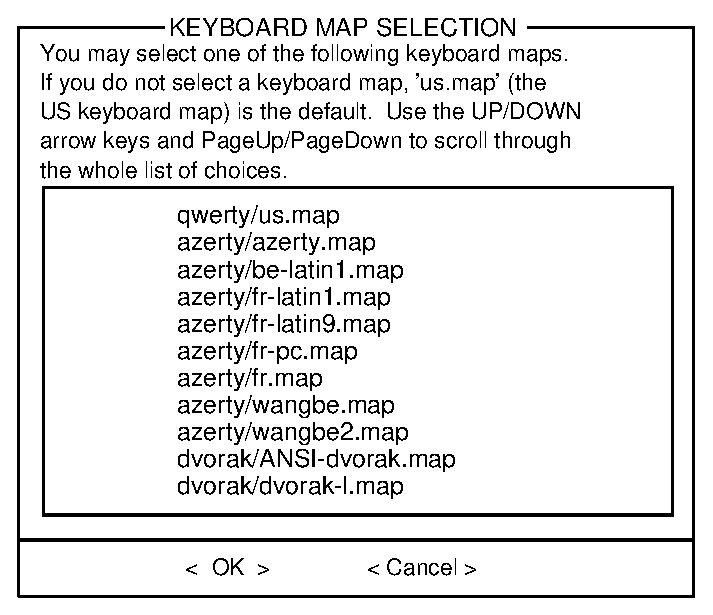
\includegraphics[width=0.8\textwidth]{images/installation/setup-keymap.eps}
  \caption{键盘映射选择}
  \label{fig:setup-keymap}
\end{figure}

\subsection{添加交换分区}
\label{sec:installation:setup:addSwap}

如果你创建了一个交换分区,那么这一步能让在你运行其它对内存敏感的活动,
诸如安装软件包之前,启用这个交换分区。交换分区是一个磁盘分区(或者是一
个文件,尽管Slackware的安装器不支持交换文件),当计算机的可用内存不足
时,会将活动的系统内存拷贝到这个分区中。通过这个方法让计算机能够在活动
内存中切换进切换出,从而能使用比计算机实际拥有的更多的内存。本步骤会将
你的交换分区加入\path{/etc/fstab}中,使之在你的操作系统中生效。参见
图\ref{fig:setup-swap}。
\begin{figure}[htpb]
  \centering
  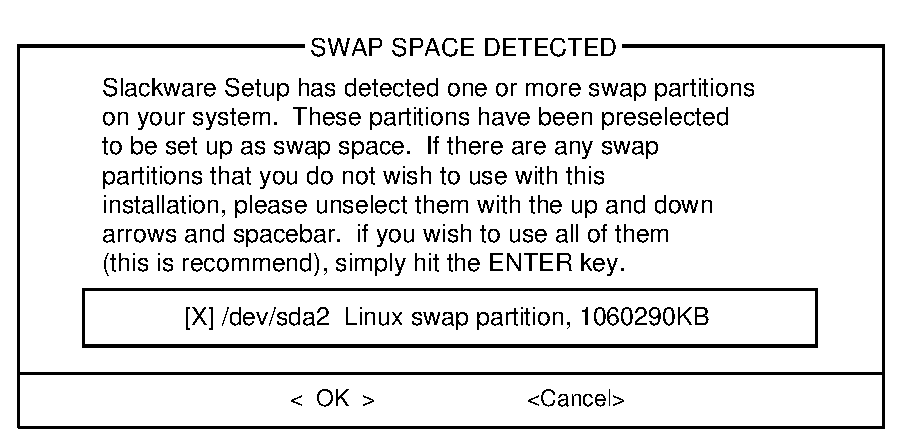
\includegraphics[width=0.8\textwidth]{images/installation/setup-swap}
  \caption{Slackware安装程序之添加交换分区}
  \label{fig:setup-swap}
\end{figure}

\subsection{选择安装位置}
\label{sec:installation:setup:target}

下一个步骤是选择根分区的位置,以及Slackware要用到的其它分区。安装程序
会提示我们选择是否使用某个分区及是否对要使用的分区格式化。如果你要安装
到一个新的分区,那么就必须先格式化。如果你要装到的分区中有你不想删除的
数据,那么不要进行格式化。例如,如果用户有一个\texttt{/home}分区,用以
存放用户数据,那么切记在安装时不要对其进行格式化。那么新安装的
Slackware就不需要对这些数据进行备份和还原了。根据使用的内核,我们可以
选择不同的文件系统,包括reiserfs、ext2、ext3、ext4、jfs及xfs等,一般而
言采用ext3或ext4即可。参见图
\ref{fig:setup-target}。
\begin{figure}[htbf]
  \centering
  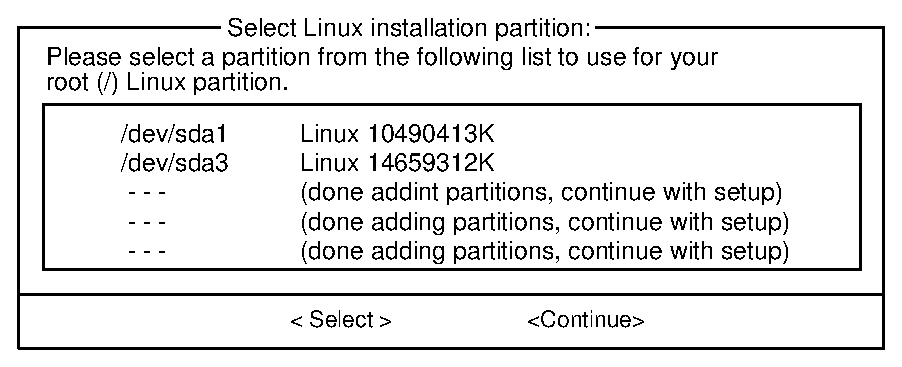
\includegraphics[width=0.8\textwidth]{images/installation/setup-target.eps}
  \caption{Slackware安装程序之选择安装位置}
  \label{fig:setup-target}
\end{figure}

进入选择安装位置后第一次选择的是安装根(/)文件系统的位置。之后,你可
以根据选择映射其它的分区到该文件系统中。(例如,你可能希望另一个分区,
如\texttt{/dev/sda3},作为你的Home文件系统。这只是一个例子,你可以按自
己的想法进行映射。)

\subsection{安装源}
\label{sec:installation:setup:source}

现在,你要告诉Slackware安装器,在哪可以找到Slackware的软件包。最常见的
方法是用Slackware安装CD或DVD,但还可以用其它的一些方式。如果你之前已经
把安装包放在之前你设置好的分区中,你可以选择从那个分区或是一个事先挂载
的文件夹中安装。(你需要先使用 mount(8) 命令挂载那个分区。参见第
\ref{chap:filesystemStructure}章以获得更多信息。)另外,Slackware还
提供了许多使基于网络的安装方法,如NFS共享、FTP、HTTP及Samba等方法。如果
你选择网络安装,Slackware会先显示提示符,让你输入TCP/IP信息。这里,我们
只讨论从DVD安装的情况,但其它的方法也很直接、简单。参见图
\ref{fig:setup-source}。
\begin{figure}[htbf]
  \centering
  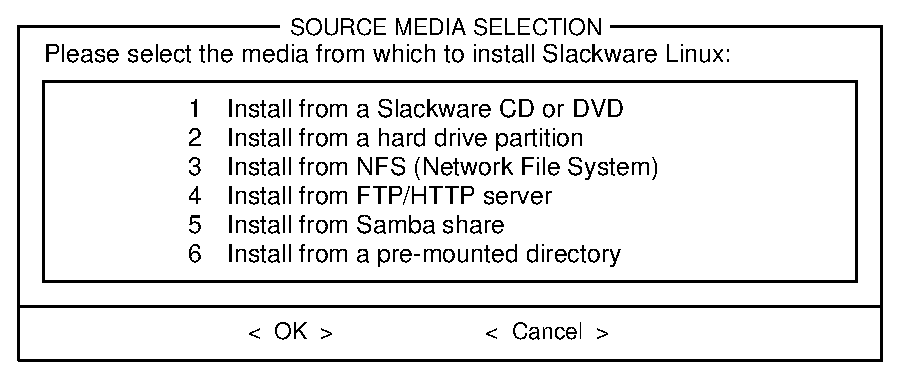
\includegraphics[width=0.8\textwidth]{images/installation/setup-source.eps}
  \caption{Slackware安装程序之选择安装源}
  \label{fig:setup-source}
\end{figure}

\subsection{选择安装包}
\label{sec:installation:setup:select}

安装器会让你选择安装哪些集合。这些集合在第
\ref{sec:installation:systemRequirements:series}节介绍过了。这个方法能
让你方便地跳过那些你可能不想安装的软件包,如在服务器上你可能不想安装X或
KDE,或者你压根就不想安装Emacs。注意``A''集合总是必须的。参见图
\ref{fig:setup-select}。
\begin{figure}[htbf]
  \centering
  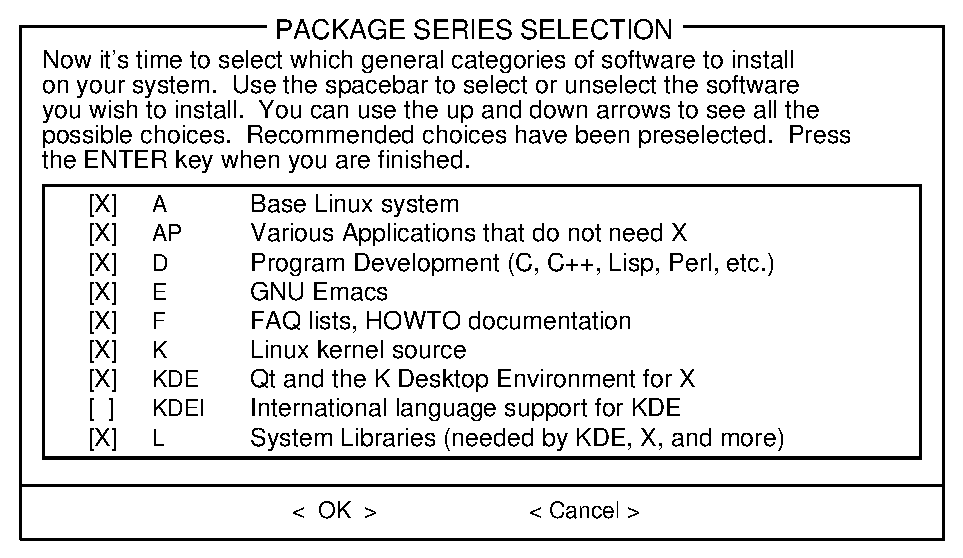
\includegraphics[width=0.8\textwidth]{images/installation/setup-select.eps}
  \caption{Slackware安装程序之选择软件包}
  \label{fig:setup-select}
\end{figure}

\subsection{安装}
\label{sec:installation:setup:install}

假设你已经完成了``target'',``source''及``select''等选项,接下来,
``install''选项让我们在软件系列中选择具体要安装的软件包。如果前面的步
骤未完成,它会提示你先完成之前的步骤。该选项可以让你从六个不同安装方法
中进行选择:\texttt{full——完全安装}、\texttt{newbie——新手安装}、
\texttt{menu——菜单安装}、\texttt{custom——自定义安装}及\texttt{tag path
  利用TAG安装}。
\begin{figure}[htpb]
  \centering
  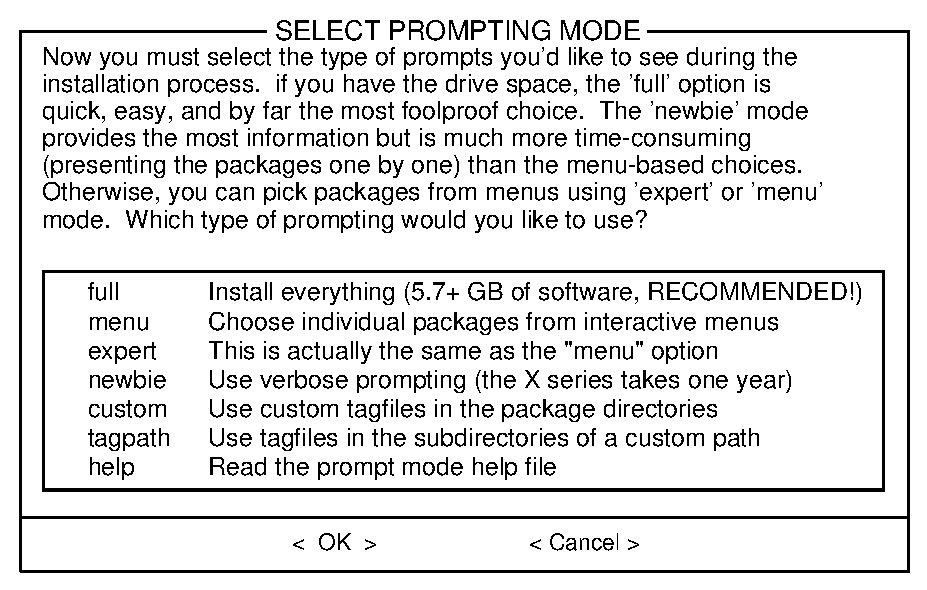
\includegraphics[width=0.8\textwidth]{images/installation/setup-install.eps}
  \caption{选择提示方式}
  \label{fig:selectPromptingMode}
\end{figure}

\texttt{full}选项会安装选择的所有系列中的所有软件包。而不会提示其它信
息。这是最容易的安装方法,因为我们不想思考到底要安装哪个软件包。当然,
这个方法用到的磁盘空间也最多。

下一个选项是\texttt{newbie}。这个选项会安装选择的系列中所有必需的软件
包。对于其它的软件包,它会给出提示符,让你选择``YES''、``NO''还是
``SKIP''。YES表示安装,NO表示不安装,SKIP则跳到下一个系列。另外,你会
看到软件包的一个描述及大小来帮助你决定是否要安装它。对于新用户来说,我
们强烈推荐使用这个选项,因为它能保证我们安装了所有必需的软件包。然而,
由于为每个软件包都显示提示符,所以速度慢。

\texttt{menu}选择是一个相对于\texttt{newbie}选项更快更高级的选项。对于
每个系列,都显示一个菜单,我们可以选择是否安装其它不是必需的软件包。必
需的软件包不会显示在这个菜单上。

对于更高级的用户,install提供了\texttt{expert}选项,这个选项能让你完全
控制想要安装的软件包。你可以不安装那些绝对需要的包,得到一个不能用的系
统。相反的,你可以精确地控制系统中安装的东西。这个选项对于新手不建议使
用,因为很可能会搬石头砸到自己的脚。

\texttt{custom}和\texttt{tag path}选项也是为高级用户而设的。这些选项让
我们能基于预先制作的tag文件来安装系统。该功能对于批量安装Slackware很有
帮助,关于使用tag文件的更多信息,请参见第
\ref{sec:packageManagement:tagfile}节。

选择了安装方法后,根据不同的方法,会有不同的响应。如果选择的是expert或
menu,那么会出现一个菜单,让你选择要安装的软件包。如果选择的是full,会
自动开始将软件包安装到目标位置中。如果选择的是newbie,在选择完可选的包
后,才会开始安装软件包。
% 对newbie的方式不太理解。

注意,安装时可能会出现磁盘空间不足,如果你选择了太多的包,而对应安装位
置的剩余空间不足,就会出现问题。最安全的方法是先选择一些包,之后再添加
其它的包。这可以通过使用slackware的包管理工具轻松完成。关于这些内容,
参见第\ref{chap:packageManagement}章。

\subsection{配置}
\label{sec:installation:setup:configure}

配置这部分会对系统进行一个基本的配置。下面出现的画面很大部分依赖于我们
安装的软件包。我们将以完全安装进行介绍。顺序可能与安装过程不太一致。
\subsubsection{创建USB启动盘}
\label{sec:installation:setup:configure:usbdisk}
很多年前,我们用软盘来创建启动盘,在其中存储启动数据。但现在软盘已经几
乎被淘汰了,一些新的计算机甚至连软驱都没有,所以,Slackware采用USB设备
来创建启动盘。基于安全的考虑,我们也建议你创建一个USB启动盘,防止之后
Slackware不能启动。如果你的机器支持从USB设备启动(现在的机器一般都支
持),那么最好在这个步骤时就创建启动盘。切记,用来创建启动盘的U盘会被
格式化,所以建议先对U盘中的数据进行备份。

另外,笔者尝试过创建USB启动盘,但4GB的U盘被格成了200MB左右,另外的空间
反而不能使用了,虽然之后没有再尝试过,但请大家作好心理准备。

\begin{figure}[htpb]
  \centering
  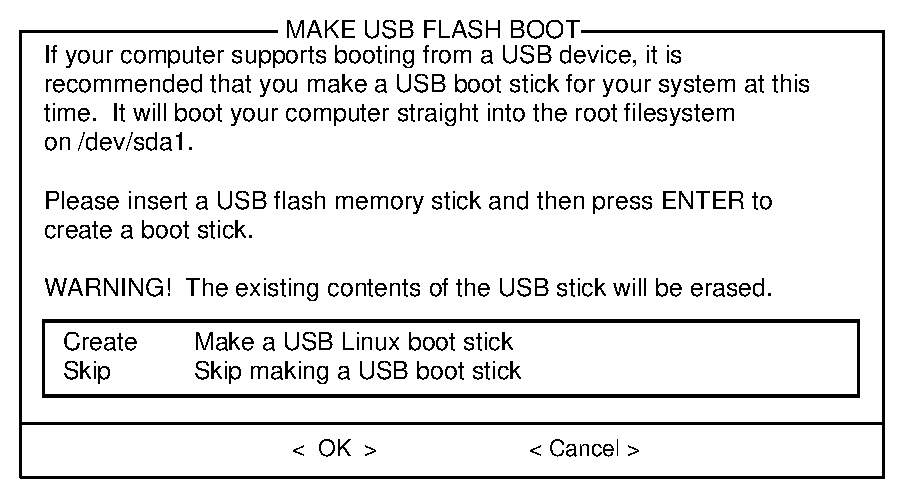
\includegraphics[width=0.8\textwidth]{images/installation/usb-boot-stick.eps}
  \caption{创建USB启动盘}
  \label{fig:usb-boot-stick}
\end{figure}

\subsubsection{LILO}
\label{sec:installation:setup:configure:lilo}这里,会提示是否安装
LILO(the LInux LOader;详情参见第\ref{sec:booting:lilo}节)
\begin{figure}[htpb]
  \centering
  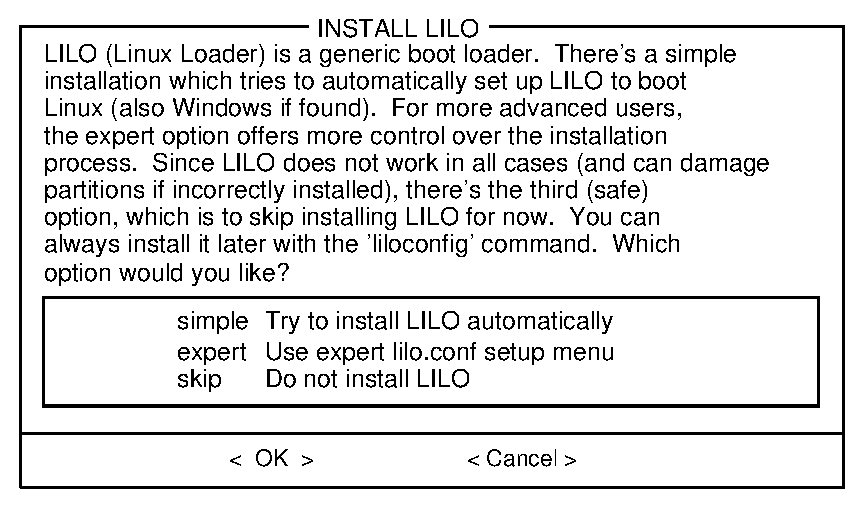
\includegraphics[width=0.8\textwidth]{images/installation/setup-lilo.eps}
  \caption{安装LILO}
  \label{fig:set-lilo}
\end{figure}
如果系统中只安装了Slackware,那么选择\texttt{simple}就可以了。如果你安
装的是双系统(或多系统),那么使用\texttt{expert}选项会更好一些。关于
双系统启动,请参见第\ref{sec:booting:lilo}节以获取更多信息。我们不推荐你
使用第三个选项\texttt{do not install},除非你知道自己在干什么,知道自
己为什么不需要安装LILO。如果选择的是\texttt{expert}选项,会有提示选择
LILO的安装位置,通常可以选择将其安装在硬盘的MBR(主引导记录)中,Linux
根分区的superblock中,或是安装在软盘上。

\subsubsection{是否使用UTF--8终端}
\label{sec:installation:setup:configure:utf8console}
从2.6.24内核起,就提供了一个标准的UTF--8终端,但由于常有一些问题,尽管
你使用的是UTF8的locale,选择默认的非UTF8文本终端会更加安全一些。
\begin{figure}[htpb]
  \centering
  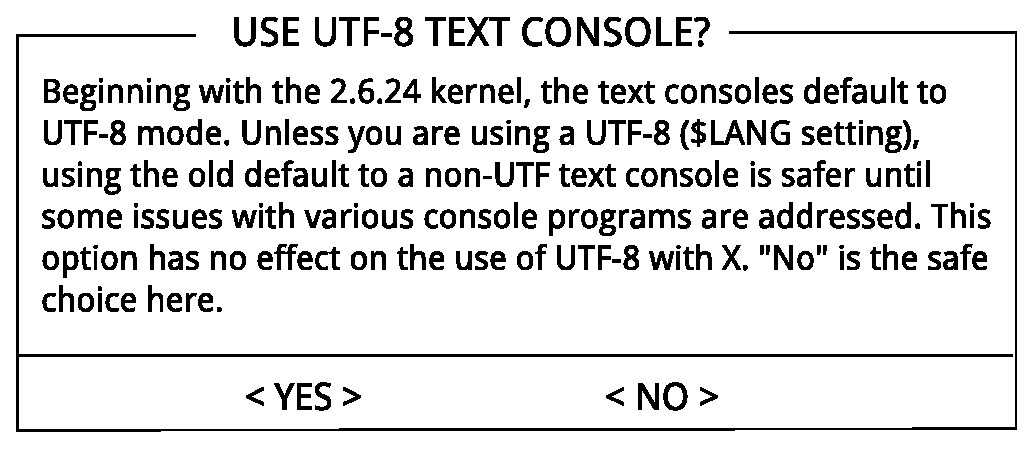
\includegraphics[width=0.8\textwidth]{images/installation/use-utf8-text-console.eps}
  \caption{是否使用UTF-8文本终端}
  \label{fig:use-utf8-text-console}
\end{figure}

\subsubsection{鼠标设置}
\label{sec:installation:setup:configure:mouse}
选择你的鼠标类型,一般选择ps/2类型或usb类型。之后会询问是否在启动时开
启\texttt{gpm\textbf{(8)}}。选择了鼠标类型后,系统会创建链接
\texttt{/dev/mouse},并指向默认的鼠标设备。如果启动后鼠标无效,可以手
动修改该文件。
\begin{figure}[htpb]
  \centering
  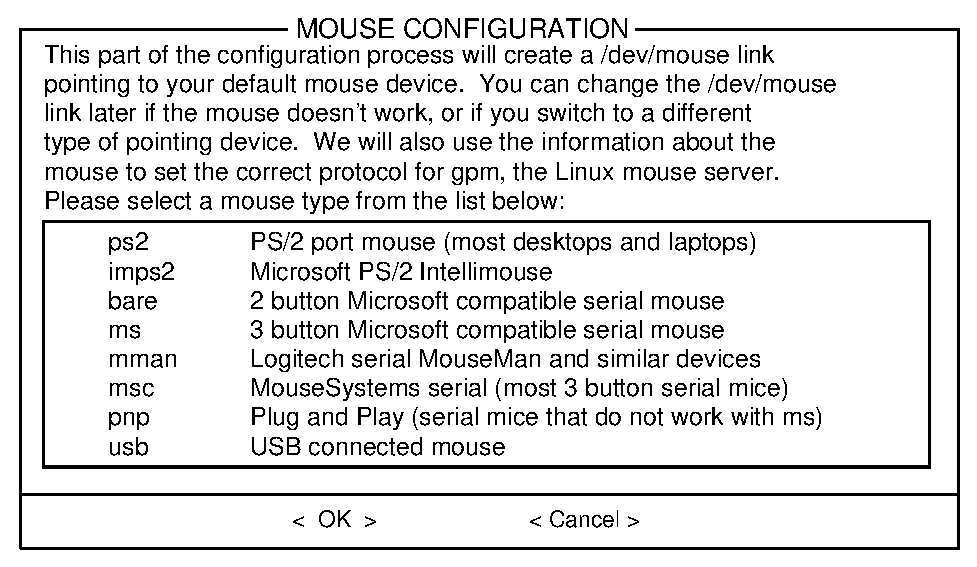
\includegraphics[width=0.8\textwidth]{images/installation/setup-mouse.eps}
  \caption{鼠标设置}
  \label{fig:setup-mouse}
\end{figure}

\subsubsection{网络设置}
\label{sec:installation:setup:configure:network}
网络设置实际上就是运行\texttt{netconfig}脚本。详情请参见第
\ref{sec:networkConfiguration:netconfig}节。

\subsubsection{选择默认启动的服务}
\label{sec:installation:setup:configure:services}
本节是选择启动时默认运行的服务。Slackware默认选择了几个服务,请根据自
己是否需要该服务进行相应的选择。如果在服务器或桌面系统上安装Slackware,
那么请关闭pcmcia服务。使用空格键进行选择及反选。请记住,开启越多的服务,
系统的安全性就越低。

如果你是新手,那么不要考虑安全性问题,尽管选就是了。
\begin{figure}[htpb]
  \centering
  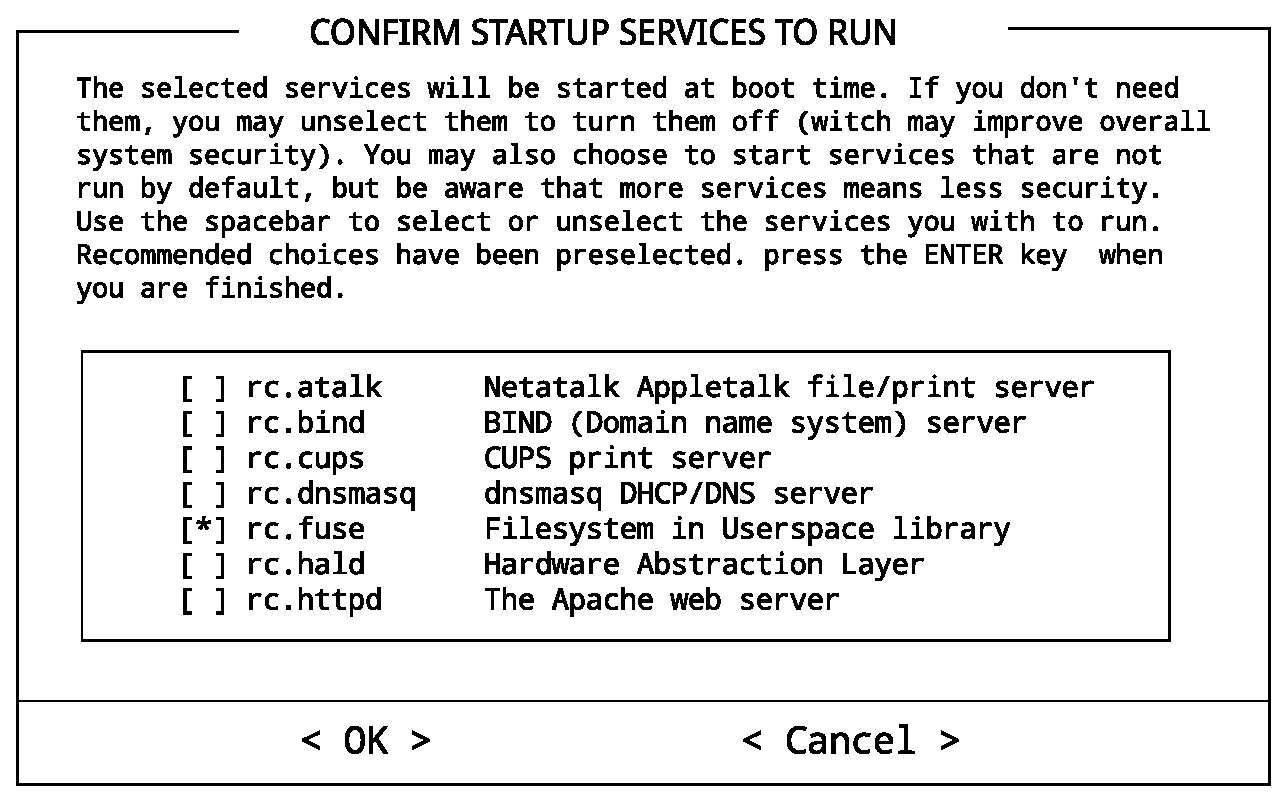
\includegraphics[width=0.8\textwidth]{images/installation/setup-services.eps}
  \caption{选择默认启动的服务}
  \label{fig:setup-services}
\end{figure}

\subsubsection{终端字体选择}
\label{sec:installation:setup:configure:consoleFont}
在该选项中可以选择终端中使用的字体。

个人建议选择``No'',因为一般而言用不到字符终端,另一方面,即使使用,使
用默认字体就能很好地显示,其它一些字体还易出现乱码。

\begin{figure}[htpb]
  \centering
  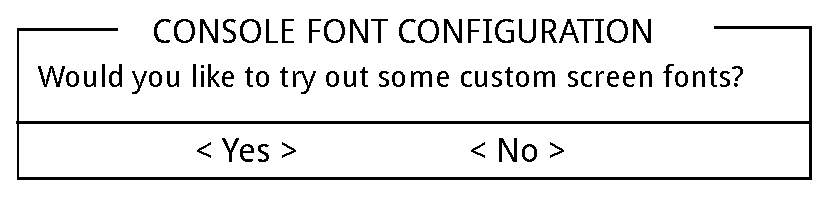
\includegraphics[width=0.8\textwidth]{images/installation/console-font.eps}
  \caption{文本终端字体选择}
  \label{fig:console-font}
\end{figure}

\subsubsection{时区选择}
\label{sec:installation:setup:configure:timezone}

这个步骤很直观,就是要你选择所在位置的时区。开始的选项是让我们选择是否
使用UTC,一般而言,选择将时钟设置为本地时间(对应选项``No'')即可。之
后选择所在的时区即可。

中国的同学们一般选择
``Asia/Shanghai'',即上海时区即可。
\begin{figure}[htpb]
  \centering
  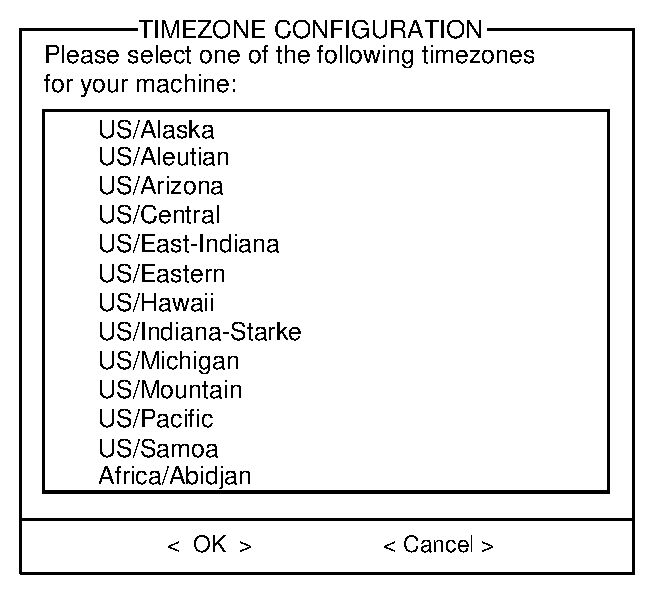
\includegraphics[width=0.8\textwidth]{images/installation/setup-timezone.eps}
  \caption{时区选择}
  \label{fig:setup-timezone}
\end{figure}

\subsubsection{X 窗口管理器}
\label{sec:installation:setup:configure:xWindowManager}

通过本节,我们就可以选择默认的X窗口管理器,参见第
\ref{chap:xconfiguration}章以获取关于X及窗口管理器的更多知识。
\begin{figure}[htpb]
  \centering
  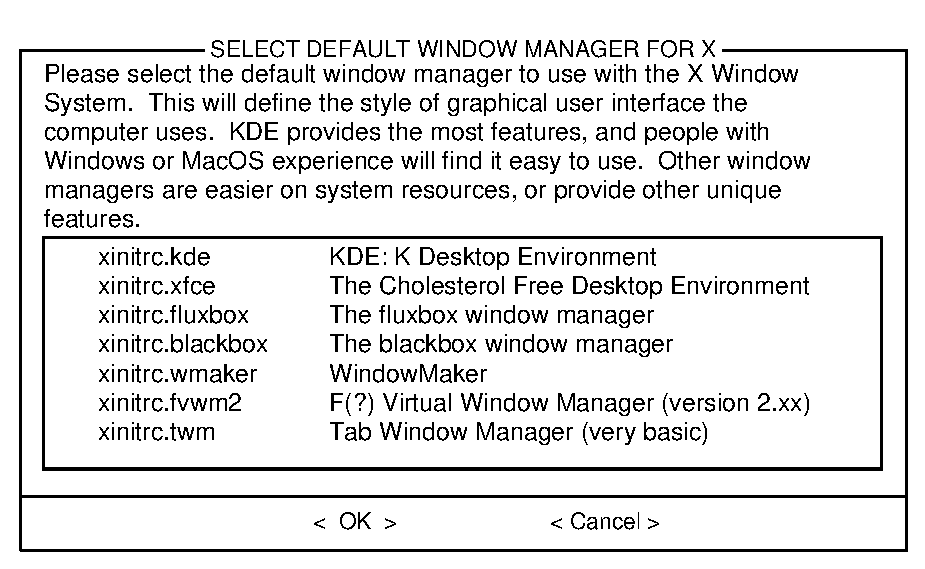
\includegraphics[width=0.8\textwidth]{images/installation/setup-xwmconfig.eps}
  \caption{选择默认的X窗口管理器}
  \label{fig:setup-xwmconfig}
\end{figure}

不管安装了什么软件包,最后一项配置是为\texttt{root}设置密码。出于安全
考虑,设置\texttt{root}密码是不会错的,但是就如Slackware中的其它东西一
样,设不设可以自己决定。





%%% Local Variables: 
%%% mode: latex
%%% TeX-master: "../SlackGuide"
%%% End: 
